\documentclass{article}
\usepackage{pgfplots, amssymb, amsmath, darkmode, fullpage, tikz,array }
\usepackage{tcolorbox}
\usetikzlibrary{positioning}

\begin{document}
\begin{center}
    \section{Parallelization}    
    \end{center}
    
    \begin{sloppypar}
        \indent{} In the grand scheme of calculations, there comes a point when there is a limiting factor in which the amount of operations per second becomes an inhibitor. As previously mentioned, the Discrete Fourier Transform has time complexity of $O(N^2)$, where $N$ is the vector size (for an $NxN$ matrix this expands to: $O(N^2N^2) = O(N^4)$). In contrast, the Fast Fourier Transform has time complexity of $O(Nlog(N))$ ($O(N^2log(N))$ when expanded to $NxN$).
    \end{sloppypar}
    \vspace{2mm}
    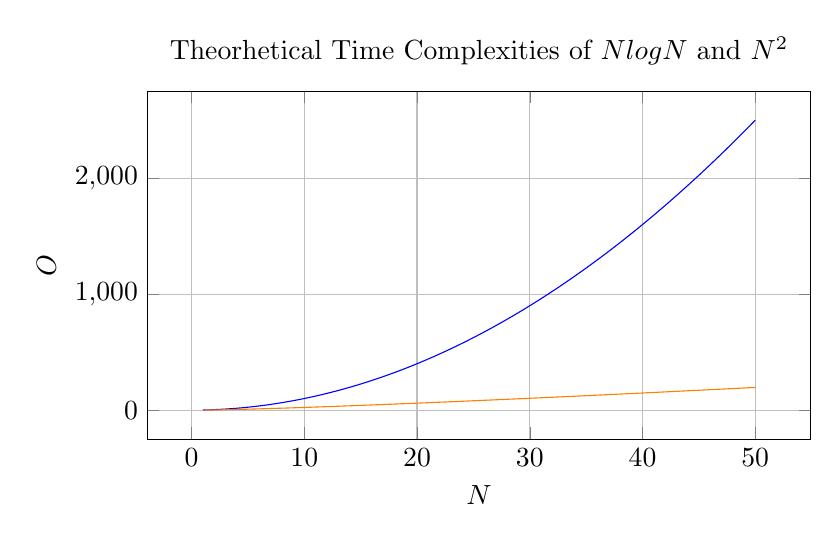
\begin{tikzpicture}
        \centering
            \begin{axis}[
                xlabel={$N$},
                ylabel={$O$},
                title={Theorhetical Time Complexities of $NlogN$ and $N^2$},
                grid=major,
                width=10cm,
                height=6cm,
                domain=1:50,
                samples=5000,
            ]
                \addplot[color=blue]{x^2};
                \addplot[color=orange]{x*ln(x)};
            \end{axis}
    \end{tikzpicture}
    \begin{sloppypar}
        \indent{}In computers there are two major processing units: Graphics processing unit and Central processing Unit. The CPU is made with a handful of cores while a modern GPU has thousands. Different processes can be offloaded to each core.
        This is where the time complexity of $O(nlogn)$ makes this so good for modern computers. We can offload the 'split' vectors/matrices to different GPU cores and compute each of these piecewise. Figure 3 below shows a rudimentary theorhetical graph of what this would look like. 
    \end{sloppypar}
    \begin{figure}[h]
    \centering
    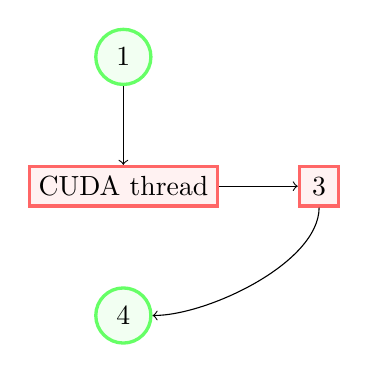
\begin{tikzpicture}[
        roundnode/.style={circle, draw=green!60, fill=green!5, very thick, minimum size=7mm},
        squarednode/.style={rectangle, draw=red!60, fill=red!5, very thick, minimum size=5mm},
        ]
        %Nodes
        \node[squarednode]      (maintopic)                              {CUDA thread};
        \node[roundnode]        (uppercircle)       [above=of maintopic] {1};
        \node[squarednode]      (rightsquare)       [right=of maintopic] {3};
        \node[roundnode]        (lowercircle)       [below=of maintopic] {4};
        
        %Lines
        \draw[->] (uppercircle.south) -- (maintopic.north);
        \draw[->] (maintopic.east) -- (rightsquare.west);
        \draw[->] (rightsquare.south) .. controls +(down:7mm) and +(right:7mm) .. (lowercircle.east);
        \end{tikzpicture}
        \caption{CUDA GPU Parallelization for FFT}
    \end{figure}
\end{document}